%
% bewegung.tex -- Begründet die Bewegung von Wirbelringen
%
% !TEX root = ../../buch.tex
% !TEX encoding = UTF-8
%
\section{Bewegung}

Bisher wurde die Bewegung eines Wirbelrings noch nicht weiter betrachtet. 
Doch wie man bereits von Rauchringen beobachten kann, bewegen sich Wirbelringe. 
Betrachtet man zunächst ein Wirbelfaden, würde auffallen, dass sich dieser nicht bewegt. 
Daher, die Bewegung entsteht durch das Schliessen der Wirbellinie in einen Kreis. 

Zugrunde zu diesem Phänomen liegt das Biot-Savart-Gesetz\cite{Wirbelringe:FuehrerdurchdieStroemungslehre}. 

\subsection{Biot-Savart-Gesetz}

Dieses Gesetz wird typischerweise in der Elektrotechnik angewendet, um das Magnetfeld von bewegten Ladungen zu beschreiben. 
Es kann auch für die Strömungsmechanik angewendet werden. 
Das Gesetz lautet 
\[
d \vec{v}
=
\frac{\Gamma}{4\pi}\frac{d \vec{l} \times \vec{r}}{\left\lvert \vec{r}^3\right\rvert }.
\]
Somit lässt sich die Geschwindigkeit eines Punktes in der Nähe eines Wirbelrings berechnen. 
Am einfachsten ist der Mittelpunkt des Kreises der Wirbellinie. 
Somit ist die Geschwindigkeit dieses Punktes
\[
\vec{v}
=
\int_{0}^{2\pi} \frac{\Gamma r}{4\pi}\frac{d \vec{l} \times \vec{r}}{\left\lvert \vec{r}^3\right\rvert }
\]
wobei r der Radius des Rings der Wirbellinie ist (und \(\Gamma\) die Zirkulation). 
Da der Kreisumfang und der Radius immer senkrecht zueinander sind, folgt 
\[
\vec{v}
=
\frac{\Gamma r}{4\pi r^3} \int_{0}^{2\pi} \hat{z} dl,
\]
wobei \(\hat{z}\) in Ausbreitungsrichtung zeigt welche senkrecht auf Radius und Kreis steht. 
Schlussendlich ergibt sich
\[
\vec{v}
=
\frac{\Gamma }{2 r^2}\hat{z}.
\]

\subsection{Bewegung eines Teilchens}

\begin{figure}
\centering
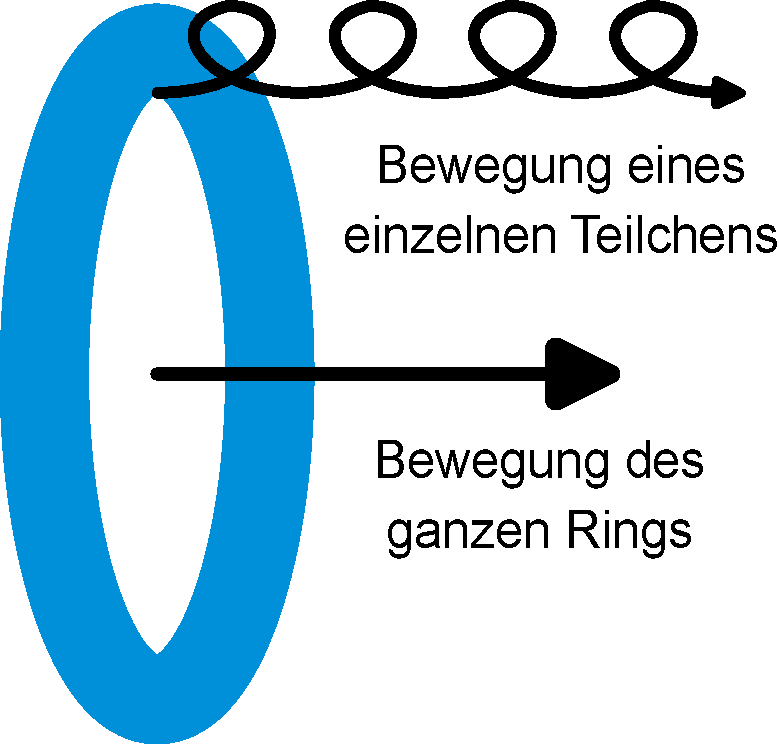
\includegraphics[width=0.4\textwidth]{papers/wirbelringe/fig/ausbreitung_teilchen.pdf}
\caption{Bewegung eines einzelnen Teilchen ToDo besseri Farb für de Ring??? \label{buch:papers:Wirbelringe:fig:ausbreitung_teilchen}}
\end{figure}

Eine interessante Kurve zeichnet sich ab, wenn man ein einzelnes Teilchen beobachtet. 
Es bildet sich eine verzogene Ellipse, welche untereinander verbunden ist. 
Die Grösse der Ellipse hängt von der Höhe der Zirkulation ab. 
Dies ist in Abbildung \ref{buch:papers:Wirbelringe:fig:ausbreitung_teilchen} dargestellt.
